\documentclass{article}
    \usepackage{subcaption}
    \usepackage{amsmath, amssymb}
    \usepackage{graphicx, float}
    \usepackage[hidelinks]{hyperref}
    \usepackage[bottom]{footmisc}
    \usepackage[margin=.8in, tmargin=.8in]{geometry}
    \usepackage{esint} % for double line integrals
    \usepackage{xcolor} % for color macros
    \usepackage{tikz}
    \usepackage{algorithm, algpseudocode}
    \newcommand{\citep}[2][]{(\cite[#1]{#2})}

    \usetikzlibrary{arrows,decorations.markings}
    \usepackage[
        backend=biber,
        % style=alphabetic,
        citestyle=authoryear,
        sorting=ynt
    ]{biblatex}
    
    \bibliography{bibliography}

    \renewcommand{\baselinestretch}{1.2}    
    \setlength\parindent{0pt}
    \setlength{\parskip}{\baselineskip}

    \newcommand{\eps}{\epsilon}
    \newcommand{\der}{\partial}
    \newcommand{\del}{\nabla}
    \newcommand{\bm}[1]{\mathbf{#1}}
    % \newcommand{\vf}[1]{\vec{\mathbf{#1}}}
    \newcommand{\vf}[1]{\mathbf{#1}}
    \newcommand{\norm}{\hat{\bm{n}}}
    \newcommand{\normal}{\mathcal{N}}
    \newcommand{\var}{\text{var}}
    \newcommand{\bx}{\vf{x}}
    \newcommand{\by}{\vf{y}}
    \newcommand{\bz}{\vf{z}}
    \newcommand{\bw}{\vf{w}}
    \newcommand{\bfu}{\vf{f}}
    \newcommand{\giv}{\ |\ }
    \newcommand{\bmu}{\pmb{\mu}}
    \newcommand{\gauss}{\mathcal{N}}
    \newcommand{\data}{\mathcal{D}}
    \newcommand{\model}{\mathcal{M}}
    \DeclareMathOperator*{\argmax}{arg\,max}
    \DeclareMathOperator*{\argmin}{arg\,min}

    \newcommand{\id}{\mathbb{I}}
    \newcommand{\de}{\text{d}}
    \newcommand{\tran}{\text{T}}
    \newcommand{\expect}{\mathbb{E}}
    \newcommand{\kl}{D_{KL}}
    \newcommand{\post}{P(\bw \giv \data)}

    \newcommand{\red}[1]{\textcolor{red}{#1}}
    \newcommand{\blue}[1]{\textcolor{blue}{#1}}
    
    \setlength\parindent{0pt}
    \captionsetup{justification=centering}
    
    \title{Reinforcement Learning}
    \date{\today}
    \author{Traiko Dinev \textless traiko.dinev@gmail.com\textgreater}

\begin{document}

\maketitle
\textit{NOTE: This partially follows Reinforcement Learning, a masters level course at the University of Edinburgh. Credit also goes to \url{https://github.com/FrancescoSaverioZuppichini/Reinforcement-Learning-Cheat-Sheet} for some great ideas. The result graphs were taken from a courseswork exercise I did for Machine Learning Practical (MLP).}

\textit{NOTE: Note this "summary" is NOT a reproduction of the course materials nor is it copied from the corresponding courses. It was entirely written and typeset from scratch.}

\textit{License: Creative Commons public license; See README.md of repository}

\section{Markov Decision Processes}
\begin{figure}[ht]
    \centering
    \begin{subfigure}{0.4\textwidth}
        \centering
        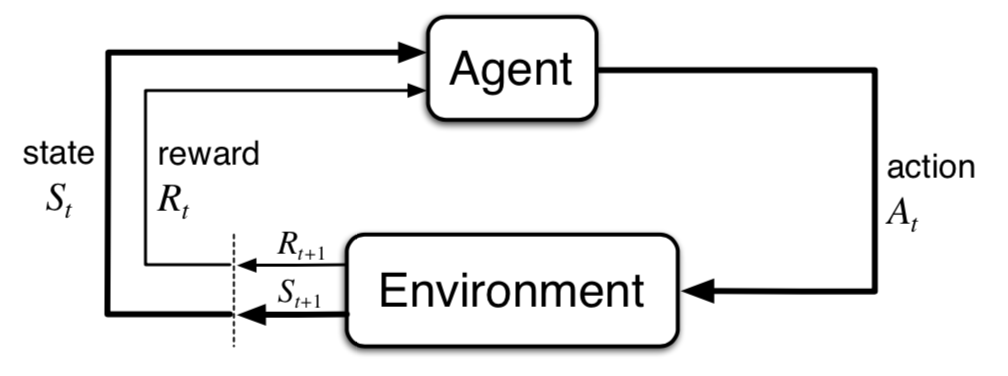
\includegraphics[width=\textwidth]{figures/agent_environment.png}
        \label{fig:agent_environment}
        \caption{Agent-Environment Interaction (from Sutton \& Barto)}
    \end{subfigure}
    %
    \centering
    \begin{subfigure}{0.25\textwidth}
        \centering
        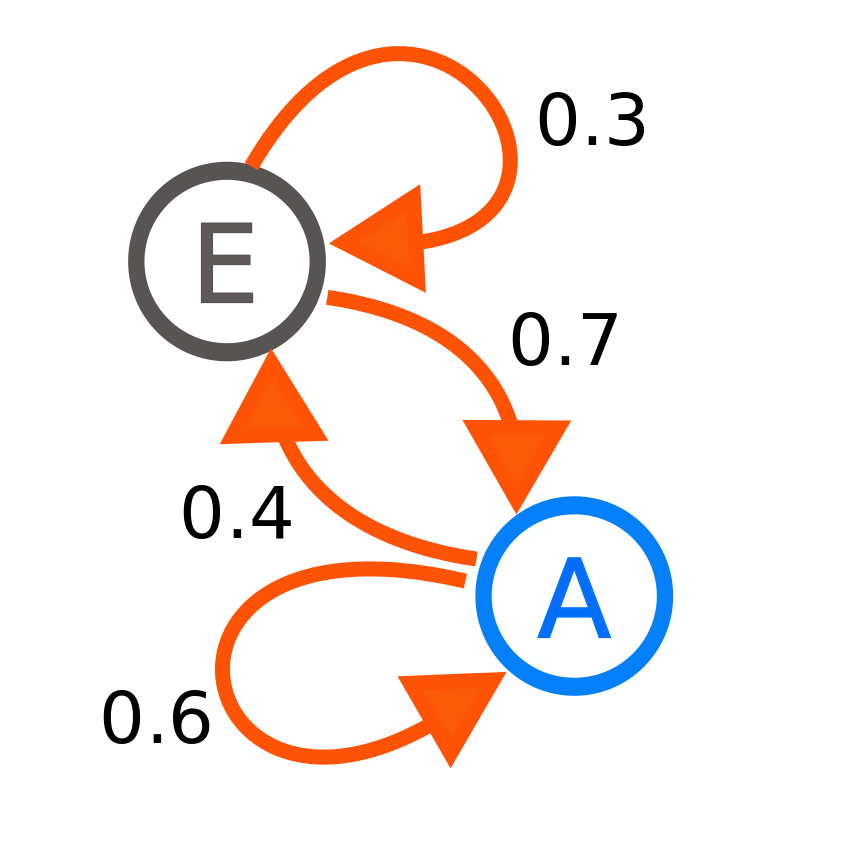
\includegraphics[width=\textwidth]{figures/Markovkate_01.png}
        \label{fig:mdp}
        \caption{An example Markov Decision Process (from wikipedia)}
    \end{subfigure}
\end{figure}


The standard reinforcement learning problem is defined as follows \citep{sutton_reinforcement_1998}; An agent is placed in an environment. At each timestep $t$ the environment is in a state $S_t = s \in \mathcal{S}$; the agent takes an action $A_t = a \in \mathcal{A}$ and receives a real-valued reward $R_{t+1} = r \in \mathbb{R}$. $S_t, A_t$ and $R_t$ are random variables. After taking an action, the state changes probabilistically, as defined in the transition function for the environment $P(S_{t+1} = s' \giv S_t = s, A_t = a)$. Our goal is to learn a policy (in most cases deterministic) $\pi \colon \mathcal{S} \to \mathcal{A}$ that for each state maps to the action that the agent would take. We define the return as:

\begin{equation}
    G_t = \sum_{k=0}^\infty \gamma^k R_{t + k + 1}
\end{equation}

where $\gamma$ is the discount parameter. The agent's goal is to maximize the expected return $\mathbb{E}[G_t \giv S_0 = s_0]$. We define the state-action value function for a policy $\pi$ as the expected return for a state and action under that policy:

\begin{equation}
    q_\pi(S_t, A_t)\ =\ \mathbb{E}_\pi\ \big[G_{t}\ |\ S_t = s, A_t = a \big]
\end{equation}

We can define an optimal policy $\pi^*$ as the policy that for each state $s \in \mathcal{S}$ and action $a \in \mathcal{A}$ satisfies $q_{\pi^*}(s,a) = q_*(s,a) > q_\pi(s, a)$ for every other policy $\pi$. The Q-function for each optimal policy is the same. We define the Bellman optimal equation \citep{sutton_reinforcement_1998}:

\begin{equation}
    q_*(s_t, a_t)\ =\ \mathbb{E}_{\pi^*}\ \big[ R_{t + 1} + \gamma\ \text{max}_{a'} q_*(s_{t+1}, a')\ |\ S_t = s_t, A_t = a_t\big]
\end{equation}

We can also define a value function $V(s_t) = \mathbb{E}\ \big[G_t\ |\ S_t = s_t \big]$ and an optimal value function in a corresponding way as the optimal Q function. The value functions also satisfy a similar Bellman equation \citep{sutton_reinforcement_1998}

In the classical reinforcement learning scenario, the optimal policy can be learned by instead learning an optimal Q function (or value function) and then computing a greedy policy:

\begin{equation}
    \pi^*(a\ |\ s) = \text{argmax}_a\ Q^*(s, a)
\end{equation}

\subsection{Q-learning and SARSA}
\textbf{Q-learning} is one of the simplest algorithms \citep{sutton_learning_1988}. The Q values are stored in a table and continuous states are discretized into buckets. After each step, the Q value for the state-action pair is updated according to the following rule:

\begin{equation}
    \begin{split}
        q(S_t, \ A_t) &= (1\ -\ \alpha)\ q(S_t,\ A_t)\ +\\
            &\alpha\ (R_{t + 1} + \gamma\ \text{max}_a\ q(S_{t+1},\ A_{t + 1}))
    \end{split}
\end{equation}

Here $\alpha$ is the learning rate, starting at $1.0$, which is exponentially decrease (anneal) by some factor (e.g. $0.995$) after each episode. The max operator approximates the Bellman optimalitiy equation.

\textbf{SARSA} \citep{a._rummery_-line_1994} is similar to Q-learning but the max operator is replaced by the action that would be taken by the current policy. The update rule is as follows:

\begin{equation}
    \begin{split}
        q(S_t,\ A_t) &= (1\ -\ \alpha)\ q(S_t, A_t)\ + \\
            &\alpha\ (R_{t+1} + \gamma q(S_{t+1}, A_{t+1}))
    \end{split}
\end{equation}

where the learning rate $\alpha$ is similarly annealed. SARSA is an example of an on-policy method, where the Q updates are computed by sampling the next action from the current policy; thus $S_{t+1}, A_{t+1}$ are computed before the update is made.

\subsection{Deep Q Learning}
Deep Q Networks (DQN) were introduced by DeepMind in their seminal paper \citep{mnih_human-level_2015}. Instead of using tables to store and update the Q values, neural networks are used. This eliminates the problem that  tables grow exponentially large with the complexity of the state. At each step, the transitions $(s_t, a_t, r_{t+1}, s_{t+1})$ are stored in what is called the \textit{experience replay}. The replay memory is also buffered with a first-in-first-out policy so as not to learn from earlier, less informative transitions. Periodically, the neural networks are trained via minibatch gradient descent. The inputs to the network are the states $\{ s_i \}_{i = 1}^N$ and the targets $y^i$ are computed as follows:

\begin{equation}
    y^i =
    \begin{cases}
        r_i\quad & \text{for final}\ s_{i+1} \\
        r_i + \gamma\ \text{max}_a Q(s_{i+1}, a; \theta) & \text{otherwise}
    \end{cases}
\end{equation}

where $\theta$ are the neural network parameters. Effectively we update the Q-value of the taken action to reflect the best possible value of Q under the current policy. 
    
Because of the max operation in equation 6, the value for Q is often overestimated. Since our predictions for Q is inherently noisy, we pick the "most overestimated" value of Q. \textcite{DBLP:journals/corr/HasseltGS15} proposed a simple solution. Instead of using one network, we now have two identical deep networks. The second network is updated to match the first every $\tau$ steps. We use the second network to compute the value updates instead of using the max operator, thus reducing the overestimation of Q values.

\subsection{Double Deep Q Networks (DDQN)}:
\begin{equation}
    y^i =
    \begin{cases}
        r_i\quad & \text{for final}\ s_{i+1} \\
        r_i + \gamma\ Q(s_{i+1}, \text{argmax}_{a'} Q(s_{i+1}, a'; \theta); \theta^-) & \text{otherwise}
    \end{cases}
\end{equation}

Where $\theta^-$ are the target network's weights. In both cases the networks are trained not after every action, but each $T$ steps taken, where the counter carries over episodes. The networks are not immediately trained, but we wait a number of iterations to let the agent gather some data by randomly exploring first.

For both algorithms, we usually suspnd training if an episode is solved, as defined in each environment. This way once we think we have reached an optimal policy $\pi^*$, we stop training until the policy fails. We do not want to "un-learn" $\pi^*$ by continuing training afterwards.

\subsection{$\epsilon$ - greedy}
The $\epsilon$-greedy exploration policy is what enables the agent to randomly \textit{explore} rather than \textit{exploit} the best found strategy so far. Instead of taking the action according to the greedy policy, as described above, with a small probability $\epsilon$ the agent takes a random action each step. $\epsilon$ is annealed similarly to $\alpha$, the learning rate, in our case by a factor of $0.995$ each episode.

See algorithm \ref{alg:dqn} for the DQN training algorithm.

\begin{algorithm}[ht]
    \begin{algorithmic}
        \State Initialize neural network with parameters $\mathbf{\theta}$
        \State counter $\gets$ 0
        \State s $\gets$ initial environment state
        \Repeat
            \State a $\gets$ $\text{argmax}_a$ Q(s, a)
            \State a $\gets$ random action with probability $\epsilon$
            
            \State Perform action and observe tuple $(s', r, \text{done})$
            \State Store tuple $(s, a, s', r, \text{done})$ in replay memory 

            \If{last environment was not solved}
                \If{counter $\geq$ start\_training}
                    \If{counter \% train\_frequency == 0}
                        \State Sample random minibatch of size $B$
                        \State Train network according to equation 6 
                    \EndIf
                \EndIf
            \EndIf
            
            \State s $\gets\ s'$

            \If{done}
                \State s $\gets$ initial environment state
                \State Reset environment
            \EndIf
            \State counter $\gets$ counter + 1
        \Until{maxEpisodes is reached}
    \end{algorithmic}
    \caption{DQN Training with $\epsilon$-greedy}
    \label{alg:dqn}
\end{algorithm}

\section{Policy Iteration}
These are a family of dynamic programming algorithms. The general Policy Iteration algorithm first evaluates a policy (Policy Evaluation) after which it updates it, taking a maximum over the values calculated in the evaluation step.

\textbf{Policy Evaluation}. Repeat until the chanages in $V(s)$, $\Delta V(s)$ are still large.
\begin{align*}
    \forall& s \in S \\
    & V(s) = \sum_a \pi(a \giv s) \sum_{s', r} P(s', r \giv s, a) \big[ r + \gamma V(s') \big]
\end{align*}

\textbf{Policy Improvement}. Repeat until the policy is unstable.
\begin{align*}
    \forall& s \in S \\
    & \pi(s) = \argmax_a \sum_{s', r} P(s', r \giv s, a) [r + \gamma V(s')]
\end{align*}

\section{Value Iteration}
This combines the above two in the same update cycle:
\begin{align*}
    \forall& s \in S \\
    & V(s) = \underbrace{\max_a \sum_{s', r}}_{\blue{\text{Note max}}} P(s', r \giv s, a) \big[ r + \gamma V(s') \big]
\end{align*}

Note the $max$ operator. This is used instead of summing over the policy $\pi(a \giv s)$. Thus we don't just evaluate the policy, but also improve it (by using the max operator). At the end we return a policy:

\begin{equation*}
    \pi(s) = \argmax_a \sum_{s', r} P(s', r \giv s, a) [r + \gamma V(s)]
\end{equation*}

\section{Monte Carlo}
Monte Carlo methods average returns over random exploratory episodes.

\begin{align*}
    &\text{Generate an episode at}\ s_0\ \text{following} \pi \\
    &\forall s, a \\
    &\quad G \gets \text{return following first occurrence of}\ s, a \\
    &\quad \text{append G to Returns(s, a)} \\
    &\quad Q(s, a) \gets \text{average(Returns(s, a))}
\end{align*}

\section{Eligibility Traces}
    \textit{TODO}

\section{Function Approximation}
This is the general case of approximating Q-functions (or V-functions) with a function, such as a deep network above. The general update rule is just a gradient descent rule. Using an MSE error, we get:

\begin{align*}
    \bm{\theta} &\gets \bm{\theta} + \alpha(V^\pi(s_t) - V_t(s_t)) \ \nabla_\bm{\theta} V_t(s_t) \\
    &= \bm{\theta} + \alpha(V^\pi(s_t) - V_t(s_t)) \ \nabla_\bm{\theta} V_t(s_t)
\end{align*}

where:

\begin{equation*}
    V_t(s_t) = f(\bm{\theta})
\end{equation*}

and $V^\pi(s_t)$ is the state value as computed in the current episode-.


\subsection{Policy Gradients Methods}
    \textit{For an excellent overview, see the tutorial by L. Weng (\cite{policy_gradient_tutorial}).}

    While SARSA tries to maximize the Q-function by using TD-errors, it still does not handle continuous actions or states very well. Indeed there are extensions of the method that better represent continuous states. Most notably, Deep Q-Networks (DQN, \cite{mnih_playing_2013}) store the Q-function as a neural network. The inputs are the states $s \in \mathcal{S}$ and the outputs -- the Q-value of the states for each action $a$. This representation, however, still relies on the environment having a discrete set of actions $\mathcal{A}$. Deep Q-Networks are similarly updated using a TD-error and the policy is chosen again using an arg max over actions.

    For continuous action spaces, such as in the swing-up problem, Deep Q-Networks suffer from the same problem as SARSA -- we need to discretize the action space, which leads to inaccuracies if there are too few buckets or high computational times if there are too many.

    We can instead look at the value of the start state $s_0$ -- $v_\pi(s_0)$ -- and try to maximize it. The policy gradient theorem states that:
    
    \begin{equation} \label{eq:policy_grad}
        \nabla v_\pi(s) = \mathbb{E}_\pi \big[
            G_t \nabla_\theta \ln \pi(a \giv s; \theta)
        \big]
    \end{equation}

    This assumes we have a parametric policy $\pi(a \giv s; \theta)$. We can now maximize $v_\pi(s_0)$ by performing a gradient \textbf{ascent} on the parameters of our policy $\theta$.

    We give a proof of the policy gradient theorem in the appendix. We combine the proof of \cite[Chapter~13]{sutton_learning_1988} with the proof of \cite{policy_gradient_tutorial} with some additional clarifications.

    \subsubsection{REINFORCE}

    % \begin{figure}[t]
    %     \centering
    %     \includegraphics[width=0.4\textwidth]{figures/reinforce_trajectory.png}
    %     \caption{Trajectory using REINFORCE with a neural network policy estimator.}
    %     \label{fig:reinforce_trajectory}
    % \end{figure}

    \autoref{eq:policy_grad} can be approximated by a single sample of $G_t$ over one episode. This is the idea behind REINFORCE:

    \begin{equation*}
        \nabla v_\pi(s) = \mathbb{E}_\pi \big[
            G_t \nabla_\theta \ln \pi(a \giv s; \theta)
        \big] \approx 
            G_t \nabla_\theta \ln \pi(a \giv s; \theta)
    \end{equation*}

    We can thus perform a simple gradient \textbf{ascent} that maximizes $v_\pi(s_0)$:

    \begin{equation*}
        \theta \gets \theta + \alpha G_t \nabla_\theta \ln \pi(A_t \giv S_t)
    \end{equation*}

    In order to apply this in practice, we average returns over the entire episode -- $\frac{1}{N} \sum_i G_i$ and additionally normalize them. We also average the gradient of the policy function in the same way. This is akin to batch gradient descent, where averaging over many samples provides a more stable gradient.

    The last key ingredient is the policy. Instead of using an $\epsilon$-greedy exploration, we use a "normal" policy:

    \begin{equation*}
        \pi(a \giv s) = \mathcal{N}(f(s; \theta), \sigma)
    \end{equation*}

    where $f(s; \theta)$ is a parametric predictor of the mean of the normal distribution. 

    \subsubsection{Deep Deterministic Policy Gradient (DDPG)}
    \begin{figure}[t]
        \centering
        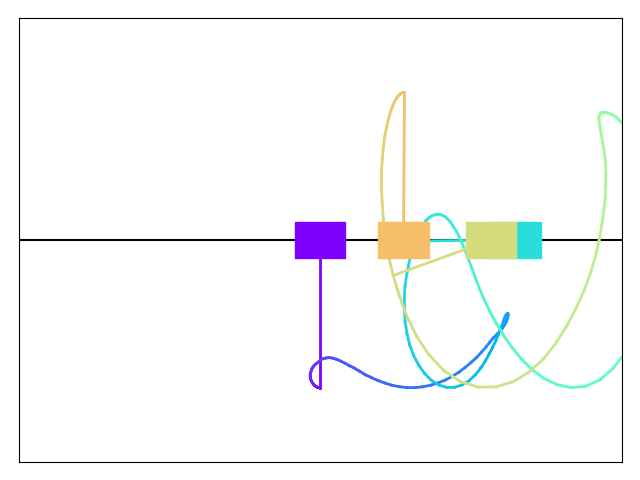
\includegraphics[width=0.4\textwidth]{figures/ddpg_trajectory.png}
        \caption{Trajectory using DDPG.}
        \label{fig:ddpg_trajectory}
    \end{figure}

    \begin{figure*}[t!]
        \vskip 5mm
        \begin{center}
        \begin{subfigure}[b]{0.4\textwidth}
        \centerline{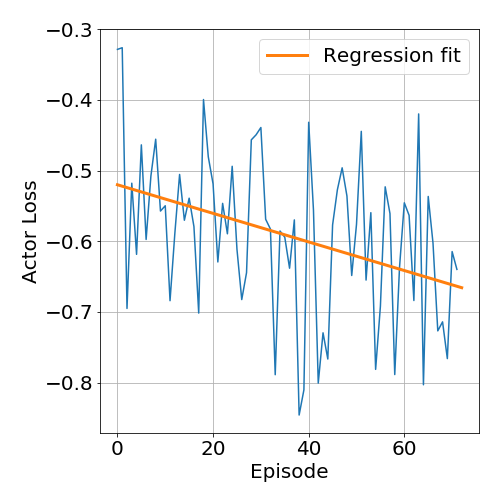
\includegraphics[width=\columnwidth]{figures/actor_loss.png}}
        % \caption{}
        % \label{fig:mountaincar_game}
        \end{subfigure}
        % 
        \begin{subfigure}[b]{0.4\textwidth}
        \centerline{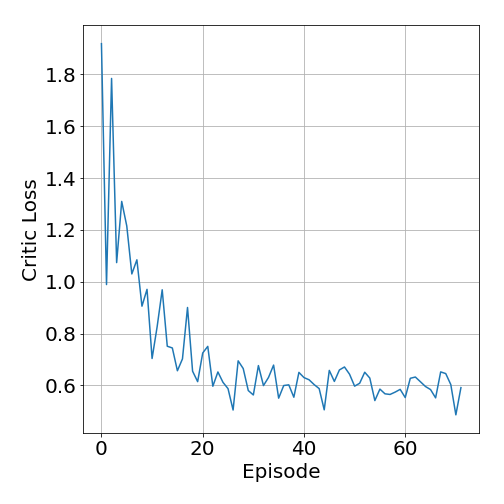
\includegraphics[width=\columnwidth]{figures/critic_loss.png}}
        % \caption{LunarLander-v2}
        % \label{fig:lunarlander_game}
        \end{subfigure}
        
        \caption{Actor and critic losses when using DDPG. The critic learns quickly, while the critic loss oscillates. We found that often the critic did not converge well and got stuck in local minima, such as immediately accelerating to the left or right. We show a fitted linear regression line for the actor loss.}
        \label{fig:ddpg_losses}
        \end{center}
        \vskip -5mm
    \end{figure*}


    In REINFORCE, we used the episodic return $G_t$ in the policy gradient. We could instead take the DQN approach (\cite{mnih_playing_2013}) and use a \textbf{critic} neural network (with parameters $\theta^Q$) to predict the $q_\pi(s, a)$ value. Additionally, we could use a deterministic policy, where $a = \pi(s; \theta^\pi)$. Again this is a neural network, called the \textbf{actor}. This slightly changes the policy gradient theorem, as proven in (\cite{pmlr-v32-silver14}). Additionally, DDPG uses the double deep-Q-learning trick (\cite{van_hasselt_deep_2015}), where the TD targets for the neural network use a second predictor network in order to reduce the variance of updates. Combining these steps, we arrive at Algorithm \ref{alg:ddpg}. We next break down the steps of the algorithm.

    We utilize an experience replay with stored transitions \\
    $(s_t, a_t, s_{t + 1}, r_t)$. At each step of the algorithm, we train over a minibatch of transitions samples from the replay. \textbf{Firstly}, we update the Q-network using a one-step TD target, similar to SARSA's update rule:

    \begin{equation} \label{eq:td_dqn}
        y_i = r_i + q(s_{i + 1}, \pi(s_{i + 1}; \theta^{\pi'}); \theta^{Q'})
    \end{equation}

    We use the target Q-value network $\theta^{Q'}$ and a one-step on-policy TD error using the target policy network $\theta^{\pi'}$. We then update the neural network using mean-squared error to match the target in \autoref{eq:td_dqn}. Thus the Q-network learns to predict the Q-values (returns) of the deterministic policy $\pi$. The policy is again a neural network, parameterized by $\theta^{\pi'}$.

    Next, we update the actor network using the deterministic policy gradient theorem (\cite{pmlr-v32-silver14}):

    \begin{equation*}
        \nabla \theta^\pi =
            \frac{1}{N} \sum_i \nabla_a Q(s, a; \theta^Q) \big|_{s = s_i, a = \pi(s_i)} \nabla_{\theta^\pi} \pi(s; \theta^\pi) \big|_{s_i}
    \end{equation*}

    This is the gradient of the Q-function:

    \begin{equation*}
        \nabla \theta^\pi =
            \frac{1}{N} \sum_i \nabla_{\theta^\pi} Q(s_i, \pi(s_i; \theta^\pi); \theta^Q)
    \end{equation*}

    Indeed this is an analog to the policy gradient theorem for deterministic policies, again using monte-carlo gradient estimation. The deterministic policy gradient theorem was introduces in \cite{pmlr-v32-silver14} and the proof is similar to that of the policy gradient theorem.

    Finally, we update the target networks parameterized by $\theta^{Q'}$ and $\theta^{\pi'}$ using an exponential moving average. This ensures that our target network is more stable:

    \begin{align*}
        \theta^{Q'} &\gets \tau \theta^Q + (1 - \tau) \theta^{Q'} \\
        \theta^{\pi'} &\gets \tau \theta^\pi + (1 - \tau) \theta^{\pi'} \\
    \end{align*}

    We applied DDPG to the inverted cart-pole system.

    We used two neural networks with one layer with $100$ neurons. Both the actor and the critic networks were trained using the Adam rule and the same $\sigma$ and $\gamma$ decay as previously. See \autoref{fig:ddpg_trajectory} for a trajectory learned by DDPG. See \autoref{fig:ddpg_losses} for an example plot of the loss functions for the actor and critic.

    We found that DDPG was by far the most difficult to converge. While the critic learned to predict Q-values well (see an example in \autoref{fig:ddpg_losses}), the actor oscillated a lot, sometimes getting stuck. Fitting a linear regression for the actor loss reveals that the overall trend is for the loss to decrease, albeit at a lower rate.

\clearpage
\printbibliography


\clearpage
\clearpage

\newcommand{\prob}{\text{P}}
\renewcommand{\vec}[1]{\mathbf{#1}}
\newcommand{\dotvec}[1]{\mathbf{\dot{#1}}}
\renewcommand{\d}[1]{\mathrm{d#1}}

\section{Appendix}
Here we provide short proofs of Lagrange's equations and the policy gradient theorem.
\subsection{Lagrangian Dynamics}
Here we give a short proof of the following theorem, known as Lagrange's equations:
\begin{equation*}
    \frac{\d{}}{\d{t}} \bigg( \frac{\partial L}{\partial \dot{\vec{q}_i}} \bigg) - \frac{\partial L}{\partial \vec{q}_i} = Q_i
\end{equation*}

The proof follows that of \cite[Section~1.5]{zak2003systems} and \cite{koskie}.

By Newton, work is defined as the force times the distance ($W = Fd$). In two (and similarly in three) dimensions, we define a generic parametric curve $C$ as:
\begin{align*}
    x &= x(t), \quad y = y(t) \\
    \vec{q} &= \langle x, y \rangle, \quad \vec{v} = \langle \dot{x}, \dot{y} \rangle \\
    0 &< t < 1
\end{align*}

If placed in a vector field $\vec{F} = \langle F_x, F_y \rangle$, the work exerted can be expressed as:

\begin{equation} \label{eq:work}
    \lim_{\Delta \vec{q} \to 0} \sum_i \vec{F} \cdot \Delta \vec{q} = 
        \int_C \vec{F} \cdot \d{\vec{q}} = 
        \int_C F_x \d{x} + \int_C F_y \d{y}
\end{equation}

% By Theorem 1 this is:

% \begin{equation} \label{eq:work}
%     W = \int_C F_x \frac{\d{x}}{\d{t}} \d{t} + \int_C F_y \frac{\d{y}}{\d{t}} \d{t} = \int_C F_x \dot{x} + F_y \dot{y}\ \d{t}
% \end{equation}

From Newton's second law, we know that:
\begin{align*}
    &\vec{F} = m \vec{a} = m \frac{\d{\vec{v}}}{\d{t}} \\
    F_x = m \ddot{x} = &m \frac{\dot{x}}{\d{t}} \quad\quad F_y = m \ddot{y} = m \frac{\dot{y}}{\d{t}}
\end{align*}

We also know that:
\begin{equation}
    \ddot{x} dx = \frac{\d{x}}{\d{t}} dx = \dot{x} \d{\dot{x}}
\end{equation}

Substituting in \autoref{eq:work}, we obtain:
\begin{equation}
    W_{AB} = \int_A^B m \dot{x} \d{\dot{x}} + \int_A^B m \dot{y} \d{\dot{y}} = m \bigg[ \frac{\dot{x}^2}{2} + \frac{\dot{y}^2}{2}  \bigg] \bigg|_A^B = \frac{m}{2} ( \norm{\dot{\vec{q}_B}}^2 - \norm{\dot{\vec{q}_A}}^2 )
\end{equation}

which is the definition of kinetic energy. Hence the work done is the difference in kinetic energies $K_A$ and $K_B$ at $A$ and $B$. This is the work-energy theorem:

\begin{equation}
    W_{AB} = K_B - K_A
\end{equation}

By the law of conservation of energy, the sum of potential and kinetic energies must remain constant. Equivalently, if the kinetic energy changes, the potential energy changes in the opposite direction.

\begin{align*}
    \Delta& K + \Delta U = 0 \\
    W &= \Delta K = - \Delta U
\end{align*}

The fundamental theorem of vector calculus states that if $\vec{U}$ is a conservative (solenoid) field, i.e. $\vec{U} = \nabla f$, then:

\begin{equation}
    \int_a^b \vec{U} \cdot \d{\vec{q}} = f(b) - f(a)
\end{equation}

We know that:
\begin{equation*}
    \Delta U = - \int_A^B \vec{F} \cdot \d{\vec{q}}
\end{equation*}

We can thus conclude that:
\begin{equation} \label{eq:fuckme}
    \vec{F}(\vec{q}) = -\nabla U (\vec{q})
\end{equation}

We can define the kinetic energy in multiple dimensions as :
\begin{equation} \label{eq:partialK}
    K = \frac{m \dot{\vec{q}}^\text{T} \dot{\vec{q}}}{2} \quad
        \frac{\partial K}{\partial\dot{\vec{q}}_i} = m \dot{\vec{q}}_i
\end{equation}

Combining \autoref{eq:partialK} with \autoref{eq:fuckme}, we obtain:
\begin{equation}
    \vec{F}_i = m \vec{a}_i = \frac{\d{}}{\d{t}} \bigg( \frac{\partial K}{\partial \dot{\vec{q}}_i} \bigg) = - \frac{\partial U}{\partial \vec{q}_i}
\end{equation}

Define the \textbf{Lagrangian} as $L = K - U$. Rearranging, we obtain:
\begin{equation*}
    \frac{\d{}}{\d{t}} \bigg( \frac{\partial L}{\partial \dot{\vec{q}}_i} \bigg) - \frac{\partial L}{\partial \vec{q}_i} = 0
\end{equation*}

where we note that:
\begin{equation*}
    \frac{\partial L}{\partial \dot{\vec{q}_i}} = \frac{\partial K}{\partial \dot{\vec{q}}_i}, \quad \quad \frac{\partial L}{\partial \vec{q}_i} = \frac{\partial U}{\partial \vec{q}_i}
\end{equation*}

An important case is when we add some energy to the system. As that adds overall energy, we can write:
\begin{equation*}
    \frac{\d{}}{\d{t}} \bigg( \frac{\partial L}{\partial \dot{\vec{q}_i}} \bigg) - \frac{\partial L}{\partial \vec{q}_i} = Q_i
\end{equation*}

where $Q_i$ is the generalized force contribution in the direction of $\vec{q}_i$.

\subsection{Policy Gradient Theorem}
Here we prove the policy gradient theorem. This proof combines that of \cite{sutton_learning_1988} with \cite{policy_gradient_tutorial} with some additional clarifications I felt were needed. We have a policy $\pi(a \giv s; \theta)$, which is parameterized by some vector $\theta$. For instance, we could use a neural network or a linear regression. Then:

\begin{equation*}
    \nabla v_\pi(s) = \mathbb{E}_\pi \big[
        G_t \nabla_\theta \ln \pi(a \giv s; \theta)
    \big]
\end{equation*}

where $\mu(s)$ is the stationary distribution of the markov chain. To define this, first we define the transition probability as a matrix. Let:

\begin{equation*}
    M_\pi[s_{t}, s_{t - 1}] =
        P(S_t = s_{t} \giv S_{t - 1} = s_{t}, \pi) 
\end{equation*}

The transition probability depends both on the transition function and the current policy $\pi$. Then assume we start at the state $s_0$. This makes the distribution of states a vector with $0$ entries everywhere and $1$ at $s_0$. The distribution over next states would be:

\begin{align*}
    p(S_0) &= [0, 0, \dots, \underbrace{0}_{\text{at} s_0}, \dots, 0]^T \\
    p(S_1) &= M p(S_0) \\
    p(S_t) &= M^t p(S_0)
\end{align*}

A stationary distribution is then the probability distribution over states as $t \to \infty$. With a little abuse of notation:

\begin{equation}
    \mu(S_\infty) = \lim_{t \to \infty} M^t p(S_0)
\end{equation}

Firstly, we need to prove the following \textbf{Lemma 1}:
\begin{align*} 
    q_\pi(s, a) &= \mathbb{E}_\pi[G_t \giv S_t = s, A_t = a] =
        \sum_{s', r} \mathbb{E}_\pi [
            G_t \giv S_t = s, A_t = a, R_{t + 1} = r, S_{t + 1} = s'
        ] P(s', r \giv s, a) \\
    &= \sum_{s', r} P(s', r \giv s, a)\ \mathbb{E}_\pi \big[
        R_{t + 1} + G_{t + 1} \giv s, a, r, s'
    \big] = \sum_{s', r} P(s', r \giv s, a) \big[r + v_\pi(s')\big]
\end{align*} 

Then we expand the definition of the value function:

\begin{align*}
    \nabla v_\pi(s) &= \nabla\mathbb{E}_\pi[G_t \giv S_t = s] =
        \nabla \bigg[\sum_a \mathbb{E}[G_t \giv S_t = s, A_t = s]\ \pi(a \giv s) \bigg]
    = \nabla \bigg[\sum_a q_\pi(s, a)\ \pi(a \giv s) \bigg] \\
    &= \sum_a \bigg[ \nabla \pi(a \giv s) q_\pi (s, a) + 
        \pi(a \giv s) \nabla q_\pi(s, a) \bigg] \\
    &= \sum_a \bigg[ \nabla \pi(a \giv s) q_\pi (s, a) + 
        \pi(a \giv s) \nabla \sum_{s', r} P(s', r \giv s, a) (r + v_\pi(s')) \bigg] \\
    &= \sum_a \bigg[ \nabla \pi(a \giv s) q_\pi (s, a) + 
        \pi(a \giv s) \sum_{s'} P(s' \giv s, a)\ \nabla v_\pi(s')) \bigg] \\
    &= \phi(s) + \sum_{s'} \sum_a \pi(a \giv s) P(s' \giv s, a) \nabla v_\pi(s')
        = \phi(s) + \sum_{s'} P(s \to s', 1) \nabla v_\pi(s') \\
\end{align*}

where $P(s \to s', 1)$ is the transition probability of getting to state $s'$ from state $s$ in one step. $\phi(s) = \sum_a \bigg[ \nabla \pi(a \giv s) q_\pi (s, a) \bigg]$. We continue to unroll the recursion, eventually arriving at the stationary distribution:

\begin{align*}
    \nabla v_\pi(s) &= \phi(s) + \sum_{s'} P(s \to s', 1) \nabla v_\pi(s') \\
    &= \phi(s) + \sum_{s'} P(s \to s', 1) \bigg[
        \phi(s') + \sum_{s''} \big[
            P(s' \to s'', 1) \nabla v_\pi(s'')
        \bigg]
    \bigg] \\
    &= \phi(s) + \sum_{s'} P(s \to s', 1)
        \phi(s') + \sum_{s''}
            P(s \to s'', 2) \nabla v_\pi(s'')\\
    &= \dots \\
    &=\sum_x \sum_{k = 0}^\infty P(s \to x, k) \phi(x) \\
    &= \sum_s \eta(x) \sum_a  q_\pi(s, a)
        \nabla_\theta \pi(a \giv s) \\
    &\propto \sum_s \frac{\eta(x)}{\sum_{\bar{x}} \eta(\bar{x})} \sum_a  q_\pi(s, a)
    \nabla_\theta \pi(a \giv s) \\
    &\propto \sum_s \mu(x) \sum_a  q_\pi(s, a)
    \nabla_\theta \pi(a \giv s) \\
    &\propto \sum_s \mu(x) \sum_a \pi(a \giv s) q_\pi(s, a) \frac{
        \nabla_\theta \pi(a \giv s)
    }{
        \pi(a \giv s)
    } \\
    &= \mathbb{E}_\pi \big[
        q_\pi(s, a) \nabla_\theta \ln \pi(a \giv s; \theta)
    \big] \\
    &= \mathbb{E}_\pi \big[
        G_t \nabla_\theta \ln \pi(a \giv s; \theta)
    \big]
\end{align*}

where on the last line we used the chain rule and the fact that $\nabla \ln x = \frac{1}{x} \nabla x$. The last step uses the following property of conditional expectations:
\begin{equation*}
    \mathbb{E}\big[ \mathbb{E} [X \giv Y] \big] = 
       \sum_y \mathbb{E} [X \giv Y = y] P(Y = y) = \mathbb{E}[X]
\end{equation*}


\end{document}
